% ============================================================
%  MeetUp — Final Project Presentation
%  Compile with: pdflatex presentation.tex
%  (Run twice for correct cross-references)
% ============================================================
\documentclass[aspectratio=169, 12pt]{beamer}

% ── Packages ─────────────────────────────────────────────
\usepackage{graphicx}
\usepackage{tikz}
\usetikzlibrary{shapes.geometric, arrows.meta, positioning, fit,
                decorations.pathreplacing, backgrounds, shadows,
                calc}
\usepackage[T1]{fontenc}
\usepackage[utf8]{inputenc}
\usepackage{lmodern}
\usepackage{listings}
\usepackage{xcolor}
\usepackage{booktabs}
\usepackage{array}
\usepackage{hyperref}
\usepackage{pgfplots}
\pgfplotsset{compat=1.18}
\usepackage{multicol}

% ── Suppress nav bar ─────────────────────────────────────
\beamertemplatenavigationsymbolsempty

% ── Custom colour palette (MeetUp brand) ─────────────────
\definecolor{MeetPrimary}{HTML}{3B82F6}   % blue-500
\definecolor{MeetDark}{HTML}{0F172A}      % slate-900
\definecolor{MeetMid}{HTML}{1E293B}       % slate-800
\definecolor{MeetLight}{HTML}{F1F5F9}     % slate-100
\definecolor{MeetAccent}{HTML}{6366F1}    % indigo-500
\definecolor{MeetGreen}{HTML}{10B981}     % emerald-500
\definecolor{MeetRed}{HTML}{EF4444}       % red-500
\definecolor{MeetGrey}{HTML}{64748B}      % slate-500
\definecolor{MeetAmber}{HTML}{F59E0B}     % amber-500
\definecolor{MeetPurple}{HTML}{8B5CF6}    % violet-500
\definecolor{MeetCyan}{HTML}{06B6D4}      % cyan-500
\definecolor{CodeBg}{HTML}{1E293B}

% ── Beamer theme customisation ───────────────────────────
\usetheme{default}
\setbeamercolor{normal text}{fg=MeetDark, bg=white}
\setbeamercolor{frametitle}{fg=white, bg=MeetDark}
\setbeamercolor{title}{fg=white}
\setbeamercolor{author}{fg=MeetLight}
\setbeamercolor{date}{fg=MeetLight}
\setbeamercolor{structure}{fg=MeetPrimary}
\setbeamercolor{block title}{fg=white, bg=MeetPrimary}
\setbeamercolor{block body}{fg=MeetDark, bg=MeetLight}
\setbeamercolor{alerted text}{fg=MeetRed}
\setbeamercolor{example text}{fg=MeetGreen}

\setbeamerfont{frametitle}{series=\bfseries, size=\large}
\setbeamerfont{title}{series=\bfseries, size=\huge}

% Frame title bar
\setbeamertemplate{frametitle}{%
  \vspace{0.25em}%
  \begin{beamercolorbox}[wd=\paperwidth, ht=2.4em, dp=0.6em, leftskip=1em]{frametitle}%
    \usebeamerfont{frametitle}\insertframetitle%
    \ifx\insertframesubtitle\empty\else%
      \\\hspace*{0.5em}{\small\color{MeetLight!70}\insertframesubtitle}%
    \fi%
  \end{beamercolorbox}%
}

% Footer
\setbeamertemplate{footline}{%
  \begin{beamercolorbox}[wd=\paperwidth, ht=1.6em, dp=0.4em]{frametitle}%
    \hspace{1em}%
    {\color{MeetLight!60}\small MeetUp --- Video Conferencing Platform}%
    \hfill%
    {\color{MeetLight!60}\small\insertframenumber\,/\,\inserttotalframenumber}%
    \hspace{1em}%
  \end{beamercolorbox}%
}

% Bullets
\setbeamertemplate{itemize item}{\color{MeetPrimary}\textbullet}
\setbeamertemplate{itemize subitem}{\color{MeetAccent}$\circ$}

% ── Code listings style ───────────────────────────────────
\lstdefinestyle{jsStyle}{
  language=JavaScript,
  backgroundcolor=\color{CodeBg},
  basicstyle=\ttfamily\footnotesize\color{white},
  keywordstyle=\color{MeetPrimary}\bfseries,
  stringstyle=\color{MeetGreen},
  commentstyle=\color{MeetGrey}\itshape,
  numbers=none,
  breaklines=true,
  frame=none,
  tabsize=2,
  showstringspaces=false,
  morekeywords={const, let, async, await, socket, io, emit, on}
}

% ── TikZ helper styles ────────────────────────────────────
\tikzset{
  box/.style={
    rectangle, rounded corners=6pt,
    minimum width=2.6cm, minimum height=1.1cm,
    text centered, font=\small\bfseries,
    drop shadow={shadow xshift=1.5pt, shadow yshift=-1.5pt,
                 fill=black!20, opacity=0.5}
  },
  smallbox/.style={
    rectangle, rounded corners=4pt,
    minimum width=2.0cm, minimum height=0.8cm,
    text centered, font=\scriptsize\bfseries,
    drop shadow={shadow xshift=1pt, shadow yshift=-1pt,
                 fill=black!15, opacity=0.4}
  },
  arrow/.style={-Stealth, thick, color=MeetPrimary},
  dasharrow/.style={-Stealth, thick, dashed, color=MeetGrey},
  label/.style={font=\scriptsize, color=MeetGrey}
}

% ═══════════════════════════════════════════════════════════
%  DOCUMENT
% ═══════════════════════════════════════════════════════════
\begin{document}

% ── 1. TITLE SLIDE ──────────────────────────────────────────
{
\setbeamertemplate{footline}{}
\begin{frame}[plain]
  \begin{tikzpicture}[remember picture, overlay]
    % Full dark background
    \fill[MeetDark] (current page.south west) rectangle (current page.north east);
    % Decorative gradient blob top-right
    \fill[MeetPrimary, opacity=0.15]
      (current page.north east) circle (5cm);
    \fill[MeetAccent, opacity=0.10]
      ([xshift=-2cm, yshift=-3cm]current page.north east) circle (4cm);
    % Decorative blob bottom-left
    \fill[MeetGreen, opacity=0.06]
      ([xshift=3cm, yshift=3cm]current page.south west) circle (4cm);
    % Bottom strip
    \fill[MeetMid]
      (current page.south west) rectangle
      ([yshift=1.5cm]current page.south east);
  \end{tikzpicture}

  \vspace{2em}
  \begin{center}
    % Logo badge
    
\begin{tikzpicture}
      \node[circle, fill=MeetPrimary, minimum size=1.8cm,
            font=\bfseries\large, text=white]{M};
    \end{tikzpicture}

    \vspace{0.6em}
    {\color{white}\Huge\bfseries MeetUp\textcolor{MeetPrimary}{.}}

    \vspace{0.3em}
    {\color{MeetLight!80}\large Real-time Peer-to-Peer Video Conferencing}

    \vspace{0.5em}
    {\color{MeetGrey}\small with Collaborative Whiteboard \& Code Editor}

    \vspace{1.0em}
    
\begin{tikzpicture}
      \draw[MeetPrimary, thick] (0,0) -- (8cm,0);
    \end{tikzpicture}

    \vspace{0.6em}
    {\color{MeetLight!60}\normalsize
      Full-Stack Web Application $\cdot$ WebRTC $\cdot$ React $\cdot$ Node.js $\cdot$ Monaco Editor}
  \end{center}
\end{frame}
}

% ── 2. THE PROBLEM ──────────────────────────────────────────
\begin{frame}{The Problem}
  \begin{columns}[T]
    \begin{column}{0.52\textwidth}
      \vspace{0.5em}
      {\large\bfseries\color{MeetDark}Starting a video call today is\ldots}
      \vspace{0.8em}
      \begin{itemize}\setlength{\itemsep}{0.6em}
        \item {\color{MeetRed}\bfseries App downloads} required (Zoom, Teams)
        \item {\color{MeetRed}\bfseries Account creation} friction for guests
        \item {\color{MeetRed}\bfseries No collaboration tools} built into calls
        \item {\color{MeetRed}\bfseries Complex IDs} that are hard to share
        \item {\color{MeetRed}\bfseries Tab switching} between IDE and call
      \end{itemize}

      \vspace{0.8em}
      \begin{block}{What we want}
        Browser-native $\cdot$ Zero installation $\cdot$\\
        Built-in Whiteboard \& IDE $\cdot$ Share a code $\cdot$ Done.
      \end{block}
    \end{column}

    \begin{column}{0.44\textwidth}
      \begin{tikzpicture}
        \node[box, fill=MeetLight, text=MeetDark, minimum width=4.2cm,
              minimum height=3.6cm, font=\normalsize] (card) at (0,0) {};

        \node[above=0.1cm of card.center, font=\small\bfseries, text=MeetGrey]
          {Traditional Flow};

        \foreach \i/\t/\c in {
          1/{Download app}/MeetRed,
          2/{Create account}/MeetRed,
          3/{Schedule meeting}/MeetGrey,
          4/{Share 15-digit ID}/MeetGrey,
          5/{Join call}/MeetGreen
        }{
          \node[rectangle, rounded corners=3pt,
                fill=\c!10, draw=\c!40, text=\c!80,
                minimum width=3.4cm, minimum height=0.55cm,
                font=\tiny\bfseries,
                yshift={(-\i*0.72cm + 1.4cm)}]
            at (card.center) {\t};
        }
      \end{tikzpicture}
    \end{column}
  \end{columns}
\end{frame}

% ── 3. WHAT IS MEETUP ───────────────────────────────────────
\begin{frame}{What is MeetUp?}
  \begin{columns}[T]
    \begin{column}{0.56\textwidth}
      \vspace{0.4em}
      {\large\bfseries MeetUp is a browser-based, all-in-one video conferencing \& collaboration platform.}

      \vspace{0.7em}
      \begin{enumerate}\setlength{\itemsep}{0.45em}
        \item Sign in with your account
        \item Click \textbf{``New Meeting''} --- get a code like \texttt{abc-def-ghi}
        \item Share the code; guests join from Dashboard
        \item P2P video, audio, and live chat
        \item \textbf{Draw together} on a collaborative whiteboard
        \item \textbf{Code together} in a full IDE with execution
        \item Review session history and chat transcripts
      \end{enumerate}

      \vspace{0.6em}
      \begin{exampleblock}{Freemium Model}
        \footnotesize
        \textbf{Free:} 30 meetings/month $\cdot$ 10 participants\\
        \textbf{Premium:} Unlimited meetings $\cdot$ 100 participants
      \end{exampleblock}
    \end{column}

    \begin{column}{0.40\textwidth}
      \vspace{0.3em}
      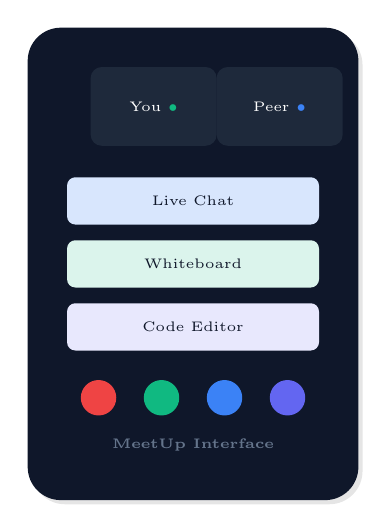
\begin{tikzpicture}
        \node[box, fill=MeetDark, text=white, minimum width=4.2cm,
              minimum height=6cm, rounded corners=12pt] (phone) at (0,0) {};

        % Video tiles
        \node[rectangle, rounded corners=4pt, fill=MeetMid,
              minimum width=1.6cm, minimum height=1.0cm,
              text=white, font=\tiny, yshift=2.0cm, xshift=-0.5cm]
          at (phone.center) {You \textcolor{MeetGreen}{$\bullet$}};
        \node[rectangle, rounded corners=4pt, fill=MeetMid,
              minimum width=1.6cm, minimum height=1.0cm,
              text=white, font=\tiny, yshift=2.0cm, xshift=1.1cm]
          at (phone.center) {Peer \textcolor{MeetPrimary}{$\bullet$}};

        % Chat bubble
        \node[rectangle, rounded corners=3pt, fill=MeetPrimary!20,
              minimum width=3.2cm, minimum height=0.6cm,
              text=MeetDark, font=\tiny, yshift=0.8cm]
          at (phone.center) {Live Chat};

        % Whiteboard
        \node[rectangle, rounded corners=3pt, fill=MeetGreen!15,
              minimum width=3.2cm, minimum height=0.6cm,
              text=MeetDark, font=\tiny, yshift=0.0cm]
          at (phone.center) {Whiteboard};

        % Code editor
        \node[rectangle, rounded corners=3pt, fill=MeetAccent!15,
              minimum width=3.2cm, minimum height=0.6cm,
              text=MeetDark, font=\tiny, yshift=-0.8cm]
          at (phone.center) {Code Editor};

        % Controls
        \foreach \i/\c in {-1.2/MeetRed, -0.4/MeetGreen, 0.4/MeetPrimary, 1.2/MeetAccent}{
          \node[circle, fill=\c, minimum size=0.45cm,
                yshift=-1.7cm, xshift=\i cm] at (phone.center) {};
        }
        \node[font=\tiny\bfseries, text=MeetGrey, yshift=-2.3cm]
          at (phone.center) {MeetUp Interface};
      \end{tikzpicture}
    \end{column}
  \end{columns}
\end{frame}

% ── 4. TECH STACK ───────────────────────────────────────────
\begin{frame}{Technology Stack}
  \vspace{0.3em}
  \begin{columns}[T]
    \begin{column}{0.48\textwidth}
      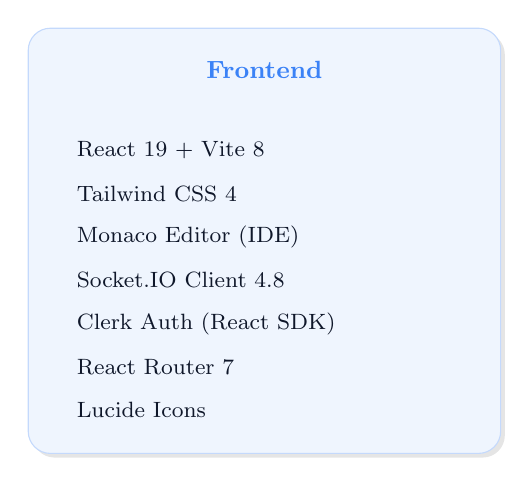
\begin{tikzpicture}
        % Frontend card
        \node[box, fill=MeetPrimary!8, draw=MeetPrimary!30,
              minimum width=6.0cm, minimum height=5.4cm,
              rounded corners=8pt] (fe) at (0,0) {};
        \node[font=\small\bfseries, text=MeetPrimary,
              anchor=north] at ([yshift=-0.3cm]fe.north)
          {Frontend};

        \foreach \i/\icon/\t in {
          1/\textcolor{MeetPrimary}{$\blacktriangleright$}/{React 19 + Vite 8},
          2/\textcolor{MeetCyan}{$\blacktriangleright$}/{Tailwind CSS 4},
          3/\textcolor{MeetAccent}{$\blacktriangleright$}/{Monaco Editor (IDE)},
          4/\textcolor{MeetGreen}{$\blacktriangleright$}/{Socket.IO Client 4.8},
          5/\textcolor{MeetAmber}{$\blacktriangleright$}/{Clerk Auth (React SDK)},
          6/\textcolor{MeetPurple}{$\blacktriangleright$}/{React Router 7},
          7/\textcolor{MeetRed}{$\blacktriangleright$}/{Lucide Icons}
        }{
          \node[font=\footnotesize, text=MeetDark, anchor=west,
                yshift={(-\i*0.55cm + 1.7cm)}]
            at ([xshift=0.4cm]fe.west) {\icon\ \t};
        }
      \end{tikzpicture}
    \end{column}

    \begin{column}{0.48\textwidth}
      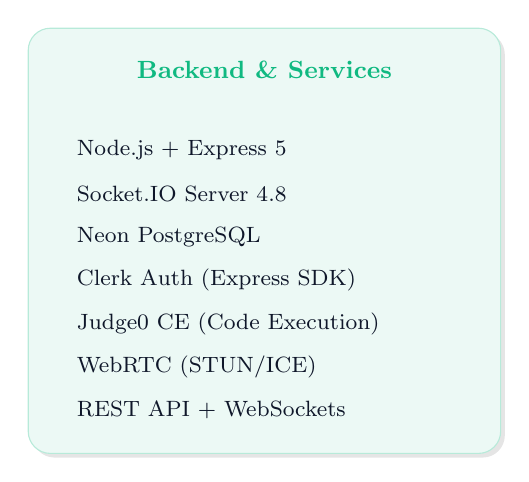
\begin{tikzpicture}
        % Backend card
        \node[box, fill=MeetGreen!8, draw=MeetGreen!30,
              minimum width=6.0cm, minimum height=5.4cm,
              rounded corners=8pt] (be) at (0,0) {};
        \node[font=\small\bfseries, text=MeetGreen,
              anchor=north] at ([yshift=-0.3cm]be.north)
          {Backend \& Services};

        \foreach \i/\icon/\t in {
          1/\textcolor{MeetGreen}{$\blacktriangleright$}/{Node.js + Express 5},
          2/\textcolor{MeetPrimary}{$\blacktriangleright$}/{Socket.IO Server 4.8},
          3/\textcolor{MeetAccent}{$\blacktriangleright$}/{Neon PostgreSQL},
          4/\textcolor{MeetAmber}{$\blacktriangleright$}/{Clerk Auth (Express SDK)},
          5/\textcolor{MeetRed}{$\blacktriangleright$}/{Judge0 CE (Code Execution)},
          6/\textcolor{MeetCyan}{$\blacktriangleright$}/{WebRTC (STUN/ICE)},
          7/\textcolor{MeetPurple}{$\blacktriangleright$}/{REST API + WebSockets}
        }{
          \node[font=\footnotesize, text=MeetDark, anchor=west,
                yshift={(-\i*0.55cm + 1.7cm)}]
            at ([xshift=0.4cm]be.west) {\icon\ \t};
        }
      \end{tikzpicture}
    \end{column}
  \end{columns}
\end{frame}

% ── 5. SYSTEM ARCHITECTURE ──────────────────────────────────
\begin{frame}{System Architecture}
  \vspace{0.2em}
  \begin{center}
  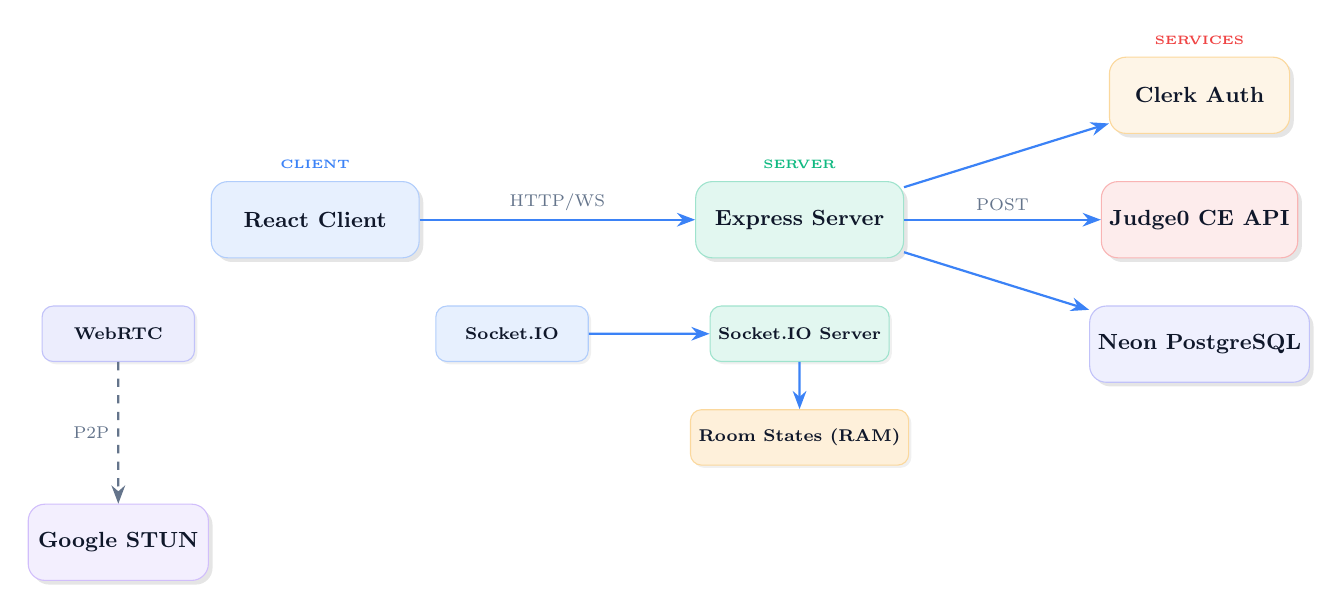
\begin{tikzpicture}[node distance=1.0cm and 1.6cm, scale=0.88, every node/.style={scale=0.88}]
    % Client Layer
    \node[box, fill=MeetPrimary!12, draw=MeetPrimary!40, text=MeetDark,
          minimum width=3.0cm] (react) {React Client};
    \node[smallbox, fill=MeetAccent!12, draw=MeetAccent!40, text=MeetDark,
          below left=0.6cm and 0.2cm of react, minimum width=2.2cm]
          (webrtc) {WebRTC};
    \node[smallbox, fill=MeetPrimary!12, draw=MeetPrimary!40, text=MeetDark,
          below right=0.6cm and 0.2cm of react, minimum width=2.2cm]
          (socketc) {Socket.IO};

    % Server Layer
    \node[box, fill=MeetGreen!12, draw=MeetGreen!40, text=MeetDark,
          right=3.5cm of react, minimum width=3.0cm]
          (express) {Express Server};
    \node[smallbox, fill=MeetGreen!12, draw=MeetGreen!40, text=MeetDark,
          below=0.6cm of express, minimum width=2.5cm]
          (socketio) {Socket.IO Server};

    % Room State
    \node[smallbox, fill=MeetAmber!15, draw=MeetAmber!40, text=MeetDark,
          below=0.6cm of socketio, minimum width=2.5cm]
          (roomstate) {Room States (RAM)};

    % External Services
    \node[box, fill=MeetRed!10, draw=MeetRed!40, text=MeetDark,
          right=2.5cm of express, minimum width=2.6cm]
          (judge0) {Judge0 CE API};
    \node[box, fill=MeetAccent!10, draw=MeetAccent!40, text=MeetDark,
          below=0.6cm of judge0, minimum width=2.6cm]
          (neon) {Neon PostgreSQL};
    \node[box, fill=MeetAmber!10, draw=MeetAmber!40, text=MeetDark,
          above=0.6cm of judge0, minimum width=2.6cm]
          (clerk) {Clerk Auth};

    % P2P
    \node[box, fill=MeetPurple!10, draw=MeetPurple!40, text=MeetDark,
          below=1.8cm of webrtc, minimum width=2.6cm]
          (stun) {Google STUN};

    % Arrows
    \draw[arrow] (react) -- node[above, label] {HTTP/WS} (express);
    \draw[arrow] (socketc) -- (socketio);
    \draw[dasharrow] (webrtc) -- node[left, label] {P2P} (stun);
    \draw[arrow] (express) -- node[above, label] {POST} (judge0);
    \draw[arrow] (express) -- (neon);
    \draw[arrow] (express) -- (clerk);
    \draw[arrow] (socketio) -- (roomstate);

    % Labels
    \node[font=\tiny\bfseries, text=MeetPrimary, above=0.05cm of react]
      {CLIENT};
    \node[font=\tiny\bfseries, text=MeetGreen, above=0.05cm of express]
      {SERVER};
    \node[font=\tiny\bfseries, text=MeetRed, above=0.05cm of clerk]
      {SERVICES};
  \end{tikzpicture}
  \end{center}
\end{frame}

% ── 6. WEBRTC SIGNALLING FLOW ───────────────────────────────
\begin{frame}{WebRTC Signalling Flow}
  \vspace{0.2em}
  \begin{center}
  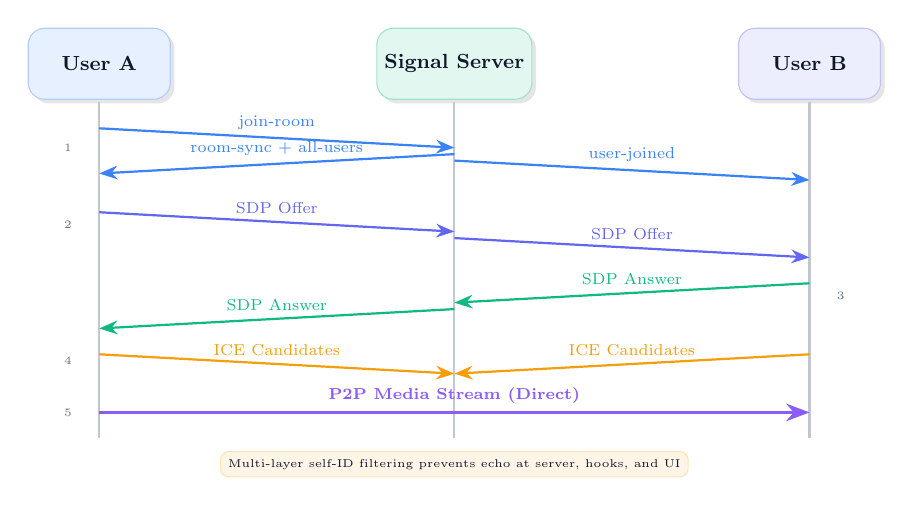
\begin{tikzpicture}[scale=0.82, every node/.style={scale=0.82}]
    % Participants
    \node[box, fill=MeetPrimary!12, draw=MeetPrimary!40, text=MeetDark,
          minimum width=2.2cm] (a) at (0,0) {User A};
    \node[box, fill=MeetGreen!12, draw=MeetGreen!40, text=MeetDark,
          minimum width=2.4cm] (s) at (5.5,0) {Signal Server};
    \node[box, fill=MeetAccent!12, draw=MeetAccent!40, text=MeetDark,
          minimum width=2.2cm] (b) at (11,0) {User B};

    % Timeline
    \draw[MeetGrey!40, thick] (0,-0.6) -- (0,-5.8);
    \draw[MeetGrey!40, thick] (5.5,-0.6) -- (5.5,-5.8);
    \draw[MeetGrey!40, thick] (11,-0.6) -- (11,-5.8);

    % Step 1
    \draw[arrow] (0,-1.0) -- node[above, font=\scriptsize] {join-room} (5.5,-1.3);
    \draw[arrow] (5.5,-1.4) -- node[above, font=\scriptsize] {room-sync + all-users} (0,-1.7);
    \draw[arrow] (5.5,-1.5) -- node[above, font=\scriptsize] {user-joined} (11,-1.8);

    % Step 2
    \draw[arrow, MeetAccent] (0,-2.3) -- node[above, font=\scriptsize]
      {SDP Offer} (5.5,-2.6);
    \draw[arrow, MeetAccent] (5.5,-2.7) -- node[above, font=\scriptsize]
      {SDP Offer} (11,-3.0);

    % Step 3
    \draw[arrow, MeetGreen] (11,-3.4) -- node[above, font=\scriptsize]
      {SDP Answer} (5.5,-3.7);
    \draw[arrow, MeetGreen] (5.5,-3.8) -- node[above, font=\scriptsize]
      {SDP Answer} (0,-4.1);

    % Step 4
    \draw[arrow, MeetAmber] (0,-4.5) -- node[above, font=\scriptsize]
      {ICE Candidates} (5.5,-4.8);
    \draw[arrow, MeetAmber] (11,-4.5) -- node[above, font=\scriptsize]
      {ICE Candidates} (5.5,-4.8);

    % Step 5
    \draw[arrow, MeetPurple, very thick] (0,-5.4) --
      node[above, font=\scriptsize\bfseries] {P2P Media Stream (Direct)}
      (11,-5.4);

    % Step labels
    \node[font=\tiny, text=MeetGrey, anchor=east] at (-0.3,-1.3) {1};
    \node[font=\tiny, text=MeetGrey, anchor=east] at (-0.3,-2.5) {2};
    \node[font=\tiny, text=MeetGrey, anchor=west] at (11.3,-3.6) {3};
    \node[font=\tiny, text=MeetGrey, anchor=east] at (-0.3,-4.6) {4};
    \node[font=\tiny, text=MeetGrey, anchor=east] at (-0.3,-5.4) {5};

    % Self-filter note
    \node[rectangle, rounded corners=3pt, fill=MeetAmber!10,
          draw=MeetAmber!30, font=\tiny, text=MeetDark,
          minimum width=4.5cm, anchor=north] at (5.5,-6.0)
      {Multi-layer self-ID filtering prevents echo at server, hooks, and UI};
  \end{tikzpicture}
  \end{center}
\end{frame}

% ── 7. DATABASE SCHEMA ──────────────────────────────────────
\begin{frame}{Database Schema}
  \framesubtitle{Neon Serverless PostgreSQL}
  \vspace{0.2em}
  \begin{center}
  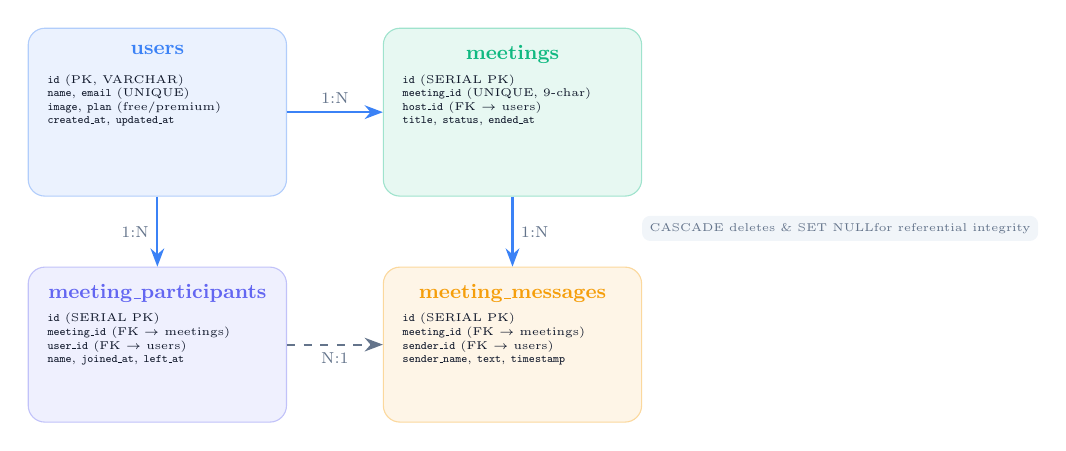
\begin{tikzpicture}[scale=0.82, every node/.style={scale=0.82}]
    % Users table
    \node[rectangle, rounded corners=6pt, fill=MeetPrimary!10,
          draw=MeetPrimary!40, minimum width=4.0cm, minimum height=2.6cm]
          (users) at (0,0) {};
    \node[font=\small\bfseries, text=MeetPrimary, anchor=north]
      at ([yshift=-0.15cm]users.north) {users};
    \node[font=\tiny, text=MeetDark, anchor=north, text width=3.4cm,
          align=left] at ([yshift=-0.6cm]users.north) {
      \texttt{id} (PK, VARCHAR)\\
      \texttt{name}, \texttt{email} (UNIQUE)\\
      \texttt{image}, \texttt{plan} (free/premium)\\
      \texttt{created\_at}, \texttt{updated\_at}
    };

    % Meetings table
    \node[rectangle, rounded corners=6pt, fill=MeetGreen!10,
          draw=MeetGreen!40, minimum width=4.0cm, minimum height=2.6cm]
          (meetings) at (5.5,0) {};
    \node[font=\small\bfseries, text=MeetGreen, anchor=north]
      at ([yshift=-0.15cm]meetings.north) {meetings};
    \node[font=\tiny, text=MeetDark, anchor=north, text width=3.4cm,
          align=left] at ([yshift=-0.6cm]meetings.north) {
      \texttt{id} (SERIAL PK)\\
      \texttt{meeting\_id} (UNIQUE, 9-char)\\
      \texttt{host\_id} (FK $\rightarrow$ users)\\
      \texttt{title}, \texttt{status}, \texttt{ended\_at}
    };

    % Participants table
    \node[rectangle, rounded corners=6pt, fill=MeetAccent!10,
          draw=MeetAccent!40, minimum width=4.0cm, minimum height=2.4cm]
          (parts) at (0,-3.6) {};
    \node[font=\small\bfseries, text=MeetAccent, anchor=north]
      at ([yshift=-0.15cm]parts.north) {meeting\_participants};
    \node[font=\tiny, text=MeetDark, anchor=north, text width=3.4cm,
          align=left] at ([yshift=-0.6cm]parts.north) {
      \texttt{id} (SERIAL PK)\\
      \texttt{meeting\_id} (FK $\rightarrow$ meetings)\\
      \texttt{user\_id} (FK $\rightarrow$ users)\\
      \texttt{name}, \texttt{joined\_at}, \texttt{left\_at}
    };

    % Messages table
    \node[rectangle, rounded corners=6pt, fill=MeetAmber!10,
          draw=MeetAmber!40, minimum width=4.0cm, minimum height=2.4cm]
          (msgs) at (5.5,-3.6) {};
    \node[font=\small\bfseries, text=MeetAmber, anchor=north]
      at ([yshift=-0.15cm]msgs.north) {meeting\_messages};
    \node[font=\tiny, text=MeetDark, anchor=north, text width=3.4cm,
          align=left] at ([yshift=-0.6cm]msgs.north) {
      \texttt{id} (SERIAL PK)\\
      \texttt{meeting\_id} (FK $\rightarrow$ meetings)\\
      \texttt{sender\_id} (FK $\rightarrow$ users)\\
      \texttt{sender\_name}, \texttt{text}, \texttt{timestamp}
    };

    % Foreign key arrows
    \draw[arrow, thick] (users.east) -- node[above, label] {1:N} (meetings.west);
    \draw[arrow, thick] (meetings.south) -- node[right, label] {1:N} (msgs.north);
    \draw[arrow, thick] (users.south) -- node[left, label] {1:N} (parts.north);
    \draw[dasharrow] (parts.east) -- node[below, label] {N:1} (msgs.west);

    % Note
    \node[rectangle, rounded corners=3pt, fill=MeetLight,
          font=\tiny, text=MeetGrey, anchor=west,
          minimum width=4cm] at (7.5,-1.8)
      {CASCADE deletes \& SET NULL\\for referential integrity};
  \end{tikzpicture}
  \end{center}
\end{frame}

% ── 8. COLLABORATIVE WHITEBOARD ─────────────────────────────
\begin{frame}{Collaborative Whiteboard}
  \framesubtitle{Real-time Drawing with Multi-tool Sync}
  \begin{columns}[T]
    \begin{column}{0.50\textwidth}
      \vspace{0.3em}
      {\small\bfseries\color{MeetDark} Dual-Canvas Architecture}
      \vspace{0.4em}
      \begin{itemize}\setlength{\itemsep}{0.35em}
        \item \textbf{Committed canvas} --- final strokes
        \item \textbf{Overlay canvas} --- live shape preview
        \item HiDPI support via \texttt{devicePixelRatio}
        \item \texttt{ResizeObserver} for responsive sizing
      \end{itemize}

      \vspace{0.5em}
      {\small\bfseries\color{MeetDark} Drawing Tools}
      \vspace{0.3em}
      \begin{itemize}\setlength{\itemsep}{0.2em}
        \item {\color{MeetPrimary}\bfseries Pen} --- freehand drawing
        \item {\color{MeetAccent}\bfseries Line / Rectangle / Circle} --- shapes
        \item {\color{MeetRed}\bfseries Eraser} --- 3$\times$ stroke width
        \item 6 colors $\cdot$ 4 stroke widths
        \item Download as PNG
      \end{itemize}
    \end{column}

    \begin{column}{0.46\textwidth}
      \vspace{0.2em}
      {\small\bfseries\color{MeetDark} 3-Event Sync System}
      \vspace{0.3em}
      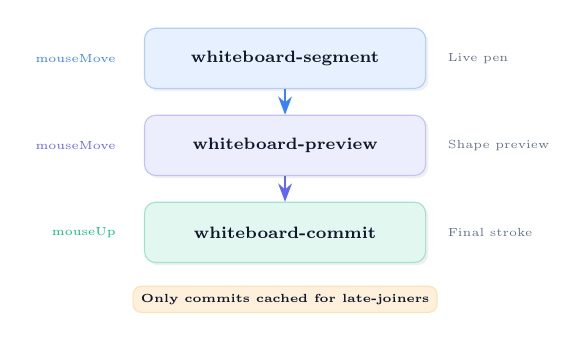
\begin{tikzpicture}[scale=0.85, every node/.style={scale=0.85}]
        % Event boxes
        \node[smallbox, fill=MeetPrimary!12, draw=MeetPrimary!40,
              text=MeetDark, minimum width=4.2cm, minimum height=0.9cm]
              (seg) at (0,0) {whiteboard-segment};
        \node[font=\tiny, text=MeetGrey, anchor=west] at (seg.east)
          {\hspace{0.2cm}Live pen};

        \node[smallbox, fill=MeetAccent!12, draw=MeetAccent!40,
              text=MeetDark, minimum width=4.2cm, minimum height=0.9cm]
              (prev) at (0,-1.3) {whiteboard-preview};
        \node[font=\tiny, text=MeetGrey, anchor=west] at (prev.east)
          {\hspace{0.2cm}Shape preview};

        \node[smallbox, fill=MeetGreen!12, draw=MeetGreen!40,
              text=MeetDark, minimum width=4.2cm, minimum height=0.9cm]
              (com) at (0,-2.6) {whiteboard-commit};
        \node[font=\tiny, text=MeetGrey, anchor=west] at (com.east)
          {\hspace{0.2cm}Final stroke};

        % Arrows
        \draw[arrow, MeetPrimary] (seg.south) -- (prev.north);
        \draw[arrow, MeetAccent] (prev.south) -- (com.north);

        % Cache indicator
        \node[rectangle, rounded corners=3pt, fill=MeetAmber!15,
              draw=MeetAmber!30, font=\tiny\bfseries, text=MeetDark,
              minimum width=3.8cm] at (0,-3.6)
          {Only commits cached for late-joiners};

        % Flow labels
        \node[font=\tiny, text=MeetPrimary, anchor=east] at ([xshift=-0.3cm]seg.west)
          {mouseMove};
        \node[font=\tiny, text=MeetAccent, anchor=east] at ([xshift=-0.3cm]prev.west)
          {mouseMove};
        \node[font=\tiny, text=MeetGreen, anchor=east] at ([xshift=-0.3cm]com.west)
          {mouseUp};
      \end{tikzpicture}
    \end{column}
  \end{columns}
\end{frame}

% ── 9. COLLABORATIVE CODE EDITOR ────────────────────────────
\begin{frame}{Collaborative Code Editor}
  \framesubtitle{VS Code--like IDE with Live Execution}
  \begin{columns}[T]
    \begin{column}{0.50\textwidth}
      \vspace{0.3em}
      {\small\bfseries\color{MeetDark} Monaco Editor Features}
      \vspace{0.3em}
      \begin{itemize}\setlength{\itemsep}{0.3em}
        \item VS Code light theme (\texttt{vs})
        \item \textbf{IntelliSense} --- 28 C++ \& 18 Java completions
        \item Snippet support with tab stops
        \item Bracket pair colorization
        \item Minimap, indentation guides
        \item Font ligatures (Geist Mono / Fira Code)
      \end{itemize}

      \vspace{0.5em}
      {\small\bfseries\color{MeetDark} Code Execution (Judge0 CE)}
      \vspace{0.3em}
      \begin{itemize}\setlength{\itemsep}{0.3em}
        \item C++ (GCC 9.2.0) --- Language ID 54
        \item Java (JDK 17.0.6) --- Language ID 91
        \item Base64 encoded submission
        \item Stdin support with live sync
        \item Execution time \& memory stats
      \end{itemize}
    \end{column}

    \begin{column}{0.46\textwidth}
      \vspace{0.2em}
      {\small\bfseries\color{MeetDark} Live Collaboration}
      \vspace{0.3em}
      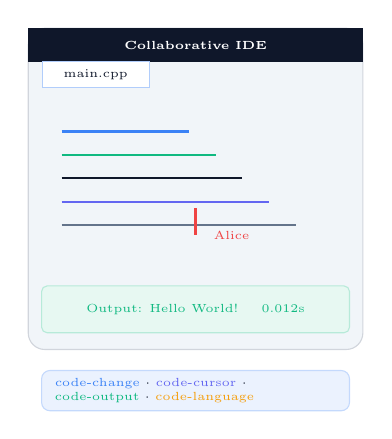
\begin{tikzpicture}[scale=0.85, every node/.style={scale=0.85}]
        % IDE mockup
        \node[rectangle, rounded corners=6pt, fill=MeetLight,
              draw=MeetGrey!30, minimum width=5.0cm,
              minimum height=4.8cm] (ide) at (0,0) {};

        % Title bar
        \node[rectangle, fill=MeetDark, minimum width=5.0cm,
              minimum height=0.5cm, rounded corners=0pt,
              anchor=north, font=\tiny\bfseries, text=white]
          at ([yshift=0cm]ide.north) {Collaborative IDE};

        % File tab
        \node[rectangle, fill=white, draw=MeetPrimary!40,
              minimum width=1.6cm, minimum height=0.35cm,
              font=\tiny, text=MeetDark, anchor=north west]
          at ([yshift=-0.5cm, xshift=-2.3cm]ide.north) {main.cpp};

        % Code lines
        \foreach \i/\c in {1/MeetPrimary, 2/MeetGreen, 3/MeetDark,
                            4/MeetAccent, 5/MeetGrey}{
          \draw[\c, thick] ([yshift={-1.2cm-\i*0.35cm}, xshift=-2.0cm]ide.north)
            -- ++({\i*0.4cm+1.5cm},0);
        }

        % Remote cursor
        \draw[MeetRed, very thick] ([yshift=-2.7cm, xshift=0cm]ide.north)
          -- ++(0, -0.4cm);
        \node[font=\tiny, text=MeetRed, anchor=west]
          at ([yshift=-3.1cm, xshift=0.15cm]ide.north) {Alice};

        % Bottom panel
        \node[rectangle, fill=MeetGreen!10, draw=MeetGreen!30,
              minimum width=4.6cm, minimum height=0.7cm,
              rounded corners=2pt, font=\tiny, text=MeetGreen,
              anchor=south] at ([yshift=0.25cm]ide.south)
          {Output: Hello World! \quad 0.012s};

        % Sync events
        \node[rectangle, rounded corners=3pt, fill=MeetPrimary!10,
              draw=MeetPrimary!30, font=\tiny, text=MeetDark,
              minimum width=4.6cm, text width=4.2cm, align=left,
              anchor=north] at ([yshift=-0.3cm]ide.south) {
          \textcolor{MeetPrimary}{code-change} $\cdot$
          \textcolor{MeetAccent}{code-cursor} $\cdot$\\
          \textcolor{MeetGreen}{code-output} $\cdot$
          \textcolor{MeetAmber}{code-language}
        };
      \end{tikzpicture}
    \end{column}
  \end{columns}
\end{frame}

% ── 10. REAL-TIME SYNC ARCHITECTURE ─────────────────────────
\begin{frame}{Real-time Sync Architecture}
  \framesubtitle{Room State Management \& Late-Joiner Recovery}
  \vspace{0.2em}
  \begin{columns}[T]
    \begin{column}{0.48\textwidth}
      {\small\bfseries\color{MeetDark} In-Memory Room State}
      \vspace{0.3em}

      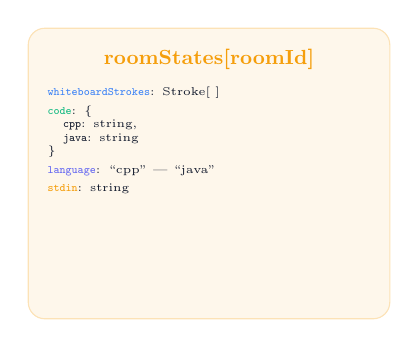
\begin{tikzpicture}[scale=0.82, every node/.style={scale=0.82}]
        \node[rectangle, rounded corners=6pt, fill=MeetAmber!8,
              draw=MeetAmber!30, minimum width=5.6cm,
              minimum height=4.5cm] (state) at (0,0) {};

        \node[font=\small\bfseries, text=MeetAmber, anchor=north]
          at ([yshift=-0.2cm]state.north) {roomStates[roomId]};

        \node[font=\tiny, text=MeetDark, anchor=north,
              text width=5.0cm, align=left]
          at ([yshift=-0.8cm]state.north) {
          \texttt{\textcolor{MeetPrimary}{whiteboardStrokes}}: Stroke[ ]\\[2pt]
          \texttt{\textcolor{MeetGreen}{code}}: \{\\
          \quad \texttt{cpp}: string,\\
          \quad \texttt{java}: string\\
          \}\\[2pt]
          \texttt{\textcolor{MeetAccent}{language}}: ``cpp'' | ``java''\\[2pt]
          \texttt{\textcolor{MeetAmber}{stdin}}: string
        };
      \end{tikzpicture}

      \vspace{0.3em}
      {\footnotesize\color{MeetGrey} Ephemeral data kept in RAM;\\
        durable data persisted to PostgreSQL.}
    \end{column}

    \begin{column}{0.48\textwidth}
      {\small\bfseries\color{MeetDark} Room Lifecycle}
      \vspace{0.3em}
      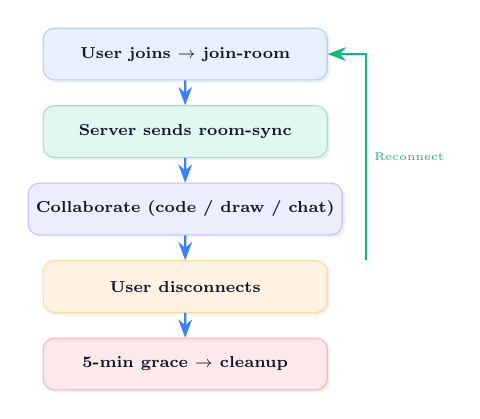
\begin{tikzpicture}[scale=0.82, every node/.style={scale=0.82}]
        % Flow
        \node[smallbox, fill=MeetPrimary!12, draw=MeetPrimary!40,
              text=MeetDark, minimum width=4.4cm] (join) at (0,0)
          {User joins $\rightarrow$ join-room};
        \node[smallbox, fill=MeetGreen!12, draw=MeetGreen!40,
              text=MeetDark, minimum width=4.4cm] (sync) at (0,-1.2)
          {Server sends room-sync};
        \node[smallbox, fill=MeetAccent!12, draw=MeetAccent!40,
              text=MeetDark, minimum width=4.4cm] (collab) at (0,-2.4)
          {Collaborate (code / draw / chat)};
        \node[smallbox, fill=MeetAmber!12, draw=MeetAmber!40,
              text=MeetDark, minimum width=4.4cm] (leave) at (0,-3.6)
          {User disconnects};
        \node[smallbox, fill=MeetRed!12, draw=MeetRed!40,
              text=MeetDark, minimum width=4.4cm] (clean) at (0,-4.8)
          {5-min grace $\rightarrow$ cleanup};

        \draw[arrow] (join) -- (sync);
        \draw[arrow] (sync) -- (collab);
        \draw[arrow] (collab) -- (leave);
        \draw[arrow] (leave) -- (clean);

        % Reconnect loop
        \draw[arrow, MeetGreen, thick]
          ([xshift=2.8cm]leave.north) |- (join.east)
          node[pos=0.25, right, font=\tiny, text=MeetGreen] {Reconnect};
      \end{tikzpicture}

      \vspace{0.3em}
      {\footnotesize\color{MeetGrey} Socket.IO: infinite reconnection\\
        with 1--5s exponential backoff.}
    \end{column}
  \end{columns}
\end{frame}

% ── 11. SOCKET EVENT MAP ────────────────────────────────────
\begin{frame}{Socket.IO Event Map}
  \framesubtitle{Complete Real-time Communication Protocol}
  \vspace{-0.2em}
  \begin{center}
  \scriptsize
  \renewcommand{\arraystretch}{0.95}
  \begin{tabular}{>{\bfseries\color{MeetPrimary}}l l >{\color{MeetGrey}}l}
    \toprule
    \textbf{\color{MeetDark}Event} & \textbf{\color{MeetDark}Direction} & \textbf{\color{MeetDark}Purpose} \\
    \midrule
    join-room          & Client $\rightarrow$ Server & Join meeting \& request state \\
    room-sync          & Server $\rightarrow$ Client & Full state recovery for late joiners \\
    \midrule
    offer / answer     & Relay (P2P)                 & WebRTC SDP exchange \\
    ice-candidate      & Relay (P2P)                 & ICE candidate trickle \\
    toggle-audio/video & Broadcast                   & Media mute / camera state changes \\
    \midrule
    send-message       & Client $\rightarrow$ Server & Chat (persisted to DB asynchronously) \\
    \midrule
    whiteboard-segment & Broadcast                   & Live incremental pen/eraser strokes \\
    whiteboard-preview & Broadcast                   & Live shape preview (line/rect/circle) \\
    whiteboard-commit  & Broadcast + Cache          & Final committed stroke (cached in RAM) \\
    whiteboard-clear   & Broadcast + Cache          & Clear all canvas strokes \\
    \midrule
    code-change        & Broadcast + Cache          & Live code edits (debounced 100ms) \\
    code-language      & Broadcast + Cache          & Language switch (C++ / Java) \\
    code-cursor        & Broadcast                  & Remote cursor tracking (debounced 80ms) \\
    code-input         & Broadcast + Cache          & Stdin updates \\
    code-output        & Broadcast                  & Judge0 execution results \\
    \midrule
    end-meeting        & Broadcast                   & Host terminates meeting for all \\
    \bottomrule
  \end{tabular}
  \end{center}
\end{frame}

% ── 12. KEY FEATURES ────────────────────────────────────────
\begin{frame}{Key Features}
  \vspace{0.3em}
  \begin{columns}[T]
    \begin{column}{0.48\textwidth}
      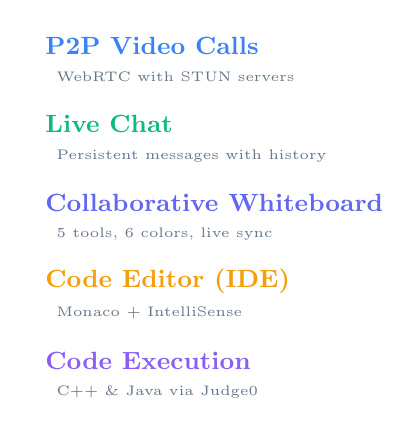
\begin{tikzpicture}
        \foreach \i/\icon/\t/\d in {
          1/{\color{MeetPrimary}$\blacksquare$}/{P2P Video Calls}/{WebRTC with STUN servers},
          2/{\color{MeetGreen}$\blacksquare$}/{Live Chat}/{Persistent messages with history},
          3/{\color{MeetAccent}$\blacksquare$}/{Collaborative Whiteboard}/{5 tools, 6 colors, live sync},
          4/{\color{MeetAmber}$\blacksquare$}/{Code Editor (IDE)}/{Monaco + IntelliSense},
          5/{\color{MeetPurple}$\blacksquare$}/{Code Execution}/{C++ \& Java via Judge0}
        }{
          \node[anchor=west, font=\small] at (0, {-\i*1.0cm+0.8cm}) {
            \icon\ \textbf{\t}
          };
          \node[anchor=west, font=\tiny, text=MeetGrey] at (0.25, {-\i*1.0cm+0.4cm}) {
            \d
          };
        }
      \end{tikzpicture}
    \end{column}

    \begin{column}{0.48\textwidth}
      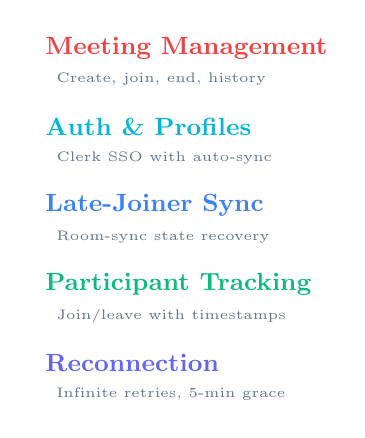
\begin{tikzpicture}
        \foreach \i/\icon/\t/\d in {
          1/{\color{MeetRed}$\blacksquare$}/{Meeting Management}/{Create, join, end, history},
          2/{\color{MeetCyan}$\blacksquare$}/{Auth \& Profiles}/{Clerk SSO with auto-sync},
          3/{\color{MeetPrimary}$\blacksquare$}/{Late-Joiner Sync}/{Room-sync state recovery},
          4/{\color{MeetGreen}$\blacksquare$}/{Participant Tracking}/{Join/leave with timestamps},
          5/{\color{MeetAccent}$\blacksquare$}/{Reconnection}/{Infinite retries, 5-min grace}
        }{
          \node[anchor=west, font=\small] at (0, {-\i*1.0cm+0.8cm}) {
            \icon\ \textbf{\t}
          };
          \node[anchor=west, font=\tiny, text=MeetGrey] at (0.25, {-\i*1.0cm+0.4cm}) {
            \d
          };
        }
      \end{tikzpicture}
    \end{column}
  \end{columns}
\end{frame}

% ── 13. ENGINEERING DECISIONS ────────────────────────────────
\begin{frame}{Engineering Decisions}
  \vspace{-0.1em}
  \begin{center}
  \scriptsize
  \renewcommand{\arraystretch}{1.12}
  \begin{tabular}{>{\bfseries\color{MeetPrimary}}p{2.8cm} p{4.6cm} >{\color{MeetGrey}}p{5.4cm}}
    \toprule
    \textbf{\color{MeetDark}Decision} & \textbf{\color{MeetDark}Choice} & \textbf{\color{MeetDark}Rationale} \\
    \midrule
    Code Editor      & Monaco Editor (\texttt{@monaco-editor/react})
                     & VS Code engine; custom IntelliSense, themes, decorations \\
    Code Execution   & Judge0 CE (Cloud API)
                     & Sandboxed execution, base64 support, zero setup \\
    Authentication   & Clerk (React + Express SDKs)
                     & Managed SSO, session tokens, auto-upsert sync \\
    Database         & Neon Serverless PostgreSQL
                     & Serverless scaling, branching, connection pooling \\
    Whiteboard Sync  & 3-event system (segment/preview/commit)
                     & Balances real-time drawing \& replay correctness \\
    Socket Lifecycle & Centralized in MeetingRoom
                     & Single persistent connection across all panels \\
    Room State       & In-memory Maps (\texttt{rooms}, \texttt{roomStates})
                     & Low-latency sync for ephemeral collaboration data \\
    Reconnection     & Infinite retries + 5-min delayed cleanup
                     & Resilient to temporary network interruptions \\
    Self-Filtering   & Multi-layer socket ID guards
                     & Eliminates echo in WebRTC video and code editing \\
    \bottomrule
  \end{tabular}
  \end{center}
\end{frame}

% ── 14. CHALLENGES & SOLUTIONS ───────────────────────────────
\begin{frame}{Challenges \& Solutions}
  \vspace{0.3em}
  \begin{columns}[T]
    \begin{column}{0.48\textwidth}
      {\small\bfseries\color{MeetRed} Challenges Faced}
      \vspace{0.4em}
      \begin{itemize}\setlength{\itemsep}{0.45em}
        \item {\color{MeetRed}\bfseries Duplicate self-video} tiles appearing
        \item {\color{MeetRed}\bfseries Socket lifecycle} conflicts between features
        \item {\color{MeetRed}\bfseries Whiteboard not live} --- only emitted on mouse-up
        \item {\color{MeetRed}\bfseries Judge0 400 errors} on special characters
        \item {\color{MeetRed}\bfseries Monaco autocomplete} clipped by containers
      \end{itemize}
    \end{column}

    \begin{column}{0.48\textwidth}
      {\small\bfseries\color{MeetGreen} Solutions Applied}
      \vspace{0.4em}
      \begin{itemize}\setlength{\itemsep}{0.45em}
        \item {\color{MeetGreen}\bfseries Multi-layer} self-ID filtering at server, hooks, and UI
        \item {\color{MeetGreen}\bfseries Centralized} socket in MeetingRoom; removed per-hook disconnect
        \item {\color{MeetGreen}\bfseries 3-event system}: segment (live) + preview + commit
        \item {\color{MeetGreen}\bfseries Base64 encoding} for source code \& stdin
        \item {\color{MeetGreen}\bfseries \texttt{fixedOverflowWidgets: true}} in Monaco config
      \end{itemize}
    \end{column}
  \end{columns}
\end{frame}

% ── 15. HOOKS ARCHITECTURE ──────────────────────────────────
\begin{frame}{Hooks-Based Architecture}
  \framesubtitle{Separation of Concerns via Custom React Hooks}
  \vspace{0.3em}
  \begin{center}
  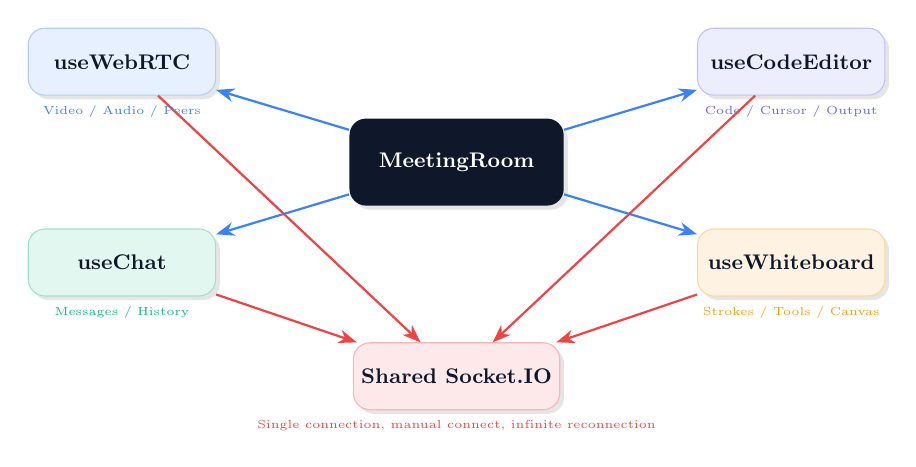
\begin{tikzpicture}[scale=0.85, every node/.style={scale=0.85}]
    % Central node
    \node[box, fill=MeetDark, text=white, minimum width=3.2cm,
          minimum height=1.3cm] (room) at (0,0) {MeetingRoom};

    % Hook nodes
    \node[box, fill=MeetPrimary!12, draw=MeetPrimary!40, text=MeetDark,
          minimum width=2.8cm, minimum height=1.0cm]
          (webrtc) at (-5, 1.5) {useWebRTC};
    \node[box, fill=MeetGreen!12, draw=MeetGreen!40, text=MeetDark,
          minimum width=2.8cm, minimum height=1.0cm]
          (chat) at (-5, -1.5) {useChat};
    \node[box, fill=MeetAccent!12, draw=MeetAccent!40, text=MeetDark,
          minimum width=2.8cm, minimum height=1.0cm]
          (code) at (5, 1.5) {useCodeEditor};
    \node[box, fill=MeetAmber!12, draw=MeetAmber!40, text=MeetDark,
          minimum width=2.8cm, minimum height=1.0cm]
          (wb) at (5, -1.5) {useWhiteboard};

    % Socket node
    \node[box, fill=MeetRed!12, draw=MeetRed!40, text=MeetDark,
          minimum width=3.0cm, minimum height=1.0cm]
          (socket) at (0, -3.2) {Shared Socket.IO};

    % Arrows from room to hooks
    \draw[arrow] (room) -- (webrtc);
    \draw[arrow] (room) -- (chat);
    \draw[arrow] (room) -- (code);
    \draw[arrow] (room) -- (wb);

    % Arrows from hooks to socket
    \draw[arrow, MeetRed] (webrtc) -- (socket);
    \draw[arrow, MeetRed] (chat) -- (socket);
    \draw[arrow, MeetRed] (code) -- (socket);
    \draw[arrow, MeetRed] (wb) -- (socket);

    % Labels
    \node[font=\tiny, text=MeetPrimary, below=0.02cm of webrtc]
      {Video / Audio / Peers};
    \node[font=\tiny, text=MeetGreen, below=0.02cm of chat]
      {Messages / History};
    \node[font=\tiny, text=MeetAccent, below=0.02cm of code]
      {Code / Cursor / Output};
    \node[font=\tiny, text=MeetAmber, below=0.02cm of wb]
      {Strokes / Tools / Canvas};
    \node[font=\tiny, text=MeetRed, below=0.02cm of socket]
      {Single connection, manual connect, infinite reconnection};
  \end{tikzpicture}
  \end{center}
\end{frame}

% ── 16. CODE EXECUTION FLOW ─────────────────────────────────
\begin{frame}{Code Execution Flow}
  \framesubtitle{Client $\rightarrow$ Server $\rightarrow$ Judge0 CE $\rightarrow$ Broadcast}
  \vspace{0.3em}
  \begin{center}
  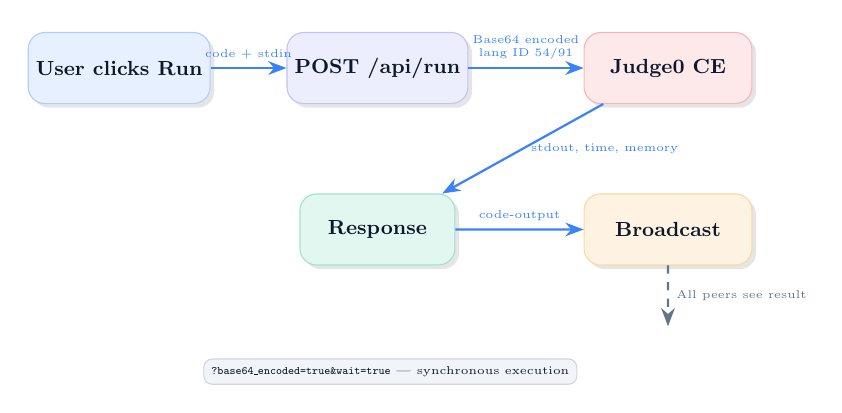
\begin{tikzpicture}[scale=0.82, every node/.style={scale=0.82}]
    % Nodes
    \node[box, fill=MeetPrimary!12, draw=MeetPrimary!40, text=MeetDark,
          minimum width=2.4cm] (user) at (0,0) {User clicks Run};
    \node[box, fill=MeetAccent!12, draw=MeetAccent!40, text=MeetDark,
          minimum width=2.4cm] (api) at (4,0) {POST /api/run};
    \node[box, fill=MeetRed!12, draw=MeetRed!40, text=MeetDark,
          minimum width=2.6cm] (j0) at (8.5,0) {Judge0 CE};
    \node[box, fill=MeetGreen!12, draw=MeetGreen!40, text=MeetDark,
          minimum width=2.4cm] (resp) at (4,-2.5) {Response};
    \node[box, fill=MeetAmber!12, draw=MeetAmber!40, text=MeetDark,
          minimum width=2.6cm] (broad) at (8.5,-2.5) {Broadcast};

    % Arrows
    \draw[arrow] (user) -- node[above, font=\tiny] {code + stdin} (api);
    \draw[arrow] (api) -- node[above, font=\tiny, text width=2cm, align=center]
      {Base64 encoded\\lang ID 54/91} (j0);
    \draw[arrow] (j0) -- node[right, font=\tiny] {stdout, time, memory} (resp);
    \draw[arrow] (resp) -- node[above, font=\tiny] {code-output} (broad);
    \draw[dasharrow] (broad) -- node[right, font=\tiny] {All peers see result} ++(0,-1.5);

    % Encoding note
    \node[rectangle, rounded corners=3pt, fill=MeetLight, draw=MeetGrey!30,
          font=\tiny, text=MeetDark, minimum width=5cm, anchor=north]
      at (4.2,-4.5) {
      \texttt{?base64\_encoded=true\&wait=true} --- synchronous execution
    };
  \end{tikzpicture}
  \end{center}
\end{frame}

% ── 17. SECURITY & PERFORMANCE ───────────────────────────────
\begin{frame}{Security \& Performance}
  \vspace{0.3em}
  \begin{columns}[T]
    \begin{column}{0.48\textwidth}
      {\small\bfseries\color{MeetPrimary} Security Measures}
      \vspace{0.5em}
      \begin{itemize}\setlength{\itemsep}{0.5em}
        \item \textbf{Clerk Auth} --- JWT-based authentication on all API routes
        \item \textbf{Auto-upsert} middleware syncs users on every request
        \item \textbf{Meeting validation} before WebRTC initialization
        \item \textbf{Capacity checks} in \texttt{join-room} (Free: 10, Premium: 100)
        \item \textbf{CORS} with dynamic origin callback
        \item \textbf{Judge0 sandboxing} --- code runs in isolated containers
      \end{itemize}
    \end{column}

    \begin{column}{0.48\textwidth}
      {\small\bfseries\color{MeetGreen} Performance Optimizations}
      \vspace{0.5em}
      \begin{itemize}\setlength{\itemsep}{0.5em}
        \item \textbf{Debounced} code changes (100ms) \& cursor updates (80ms)
        \item \textbf{In-memory state} avoids DB for ephemeral data
        \item \textbf{WebSocket-first} transport with polling fallback
        \item \textbf{Stale cursor cleanup} every 15 seconds
        \item \textbf{Lazy state init} via \texttt{getOrCreateRoomState()}
        \item \textbf{Asynchronous} message persistence to DB
      \end{itemize}
    \end{column}
  \end{columns}
\end{frame}

% ── 18. ROADMAP ──────────────────────────────────────────────
\begin{frame}{Future Roadmap}
  \vspace{0.3em}
  \begin{center}
  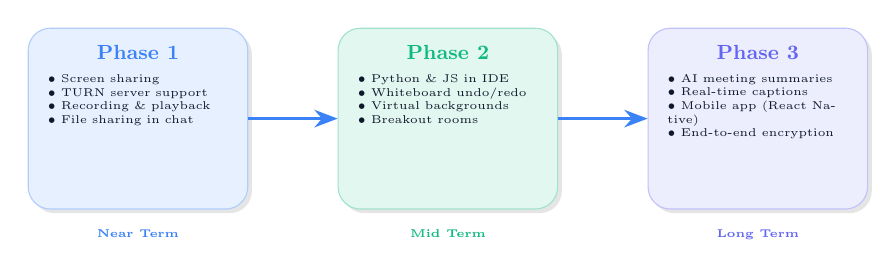
\begin{tikzpicture}[scale=0.82, every node/.style={scale=0.82}]
    % Phase boxes
    \node[box, fill=MeetPrimary!12, draw=MeetPrimary!40, text=MeetDark,
          minimum width=3.4cm, minimum height=2.8cm, rounded corners=8pt]
          (p1) at (0,0) {};
    \node[font=\small\bfseries, text=MeetPrimary, anchor=north]
      at ([yshift=-0.15cm]p1.north) {Phase 1};
    \node[font=\tiny, text=MeetDark, text width=2.8cm, align=left,
          anchor=north] at ([yshift=-0.6cm]p1.north) {
      $\bullet$ Screen sharing\\
      $\bullet$ TURN server support\\
      $\bullet$ Recording \& playback\\
      $\bullet$ File sharing in chat
    };

    \node[box, fill=MeetGreen!12, draw=MeetGreen!40, text=MeetDark,
          minimum width=3.4cm, minimum height=2.8cm, rounded corners=8pt]
          (p2) at (4.8,0) {};
    \node[font=\small\bfseries, text=MeetGreen, anchor=north]
      at ([yshift=-0.15cm]p2.north) {Phase 2};
    \node[font=\tiny, text=MeetDark, text width=2.8cm, align=left,
          anchor=north] at ([yshift=-0.6cm]p2.north) {
      $\bullet$ Python \& JS in IDE\\
      $\bullet$ Whiteboard undo/redo\\
      $\bullet$ Virtual backgrounds\\
      $\bullet$ Breakout rooms
    };

    \node[box, fill=MeetAccent!12, draw=MeetAccent!40, text=MeetDark,
          minimum width=3.4cm, minimum height=2.8cm, rounded corners=8pt]
          (p3) at (9.6,0) {};
    \node[font=\small\bfseries, text=MeetAccent, anchor=north]
      at ([yshift=-0.15cm]p3.north) {Phase 3};
    \node[font=\tiny, text=MeetDark, text width=2.8cm, align=left,
          anchor=north] at ([yshift=-0.6cm]p3.north) {
      $\bullet$ AI meeting summaries\\
      $\bullet$ Real-time captions\\
      $\bullet$ Mobile app (React Native)\\
      $\bullet$ End-to-end encryption
    };

    % Arrows
    \draw[arrow, very thick] (p1.east) -- (p2.west);
    \draw[arrow, very thick] (p2.east) -- (p3.west);

    % Labels
    \node[font=\tiny\bfseries, text=MeetPrimary, below=0.15cm of p1]
      {Near Term};
    \node[font=\tiny\bfseries, text=MeetGreen, below=0.15cm of p2]
      {Mid Term};
    \node[font=\tiny\bfseries, text=MeetAccent, below=0.15cm of p3]
      {Long Term};
  \end{tikzpicture}
  \end{center}
\end{frame}

% ── 19. THANK YOU ────────────────────────────────────────────
{
\setbeamertemplate{footline}{}
\begin{frame}[plain]
  \begin{tikzpicture}[remember picture, overlay]
    \fill[MeetDark] (current page.south west) rectangle (current page.north east);
    \fill[MeetPrimary, opacity=0.12]
      ([xshift=-4cm]current page.north east) circle (6cm);
    \fill[MeetAccent, opacity=0.08]
      ([xshift=4cm, yshift=2cm]current page.south west) circle (5cm);
    \fill[MeetGreen, opacity=0.06]
      ([xshift=-2cm, yshift=-1cm]current page.north west) circle (3cm);
  \end{tikzpicture}

  \begin{center}
    \vspace{2.5em}

    % Logo
    
\begin{tikzpicture}
      \node[circle, fill=MeetPrimary, minimum size=2.0cm,
            font=\bfseries\Large, text=white]{M};
    \end{tikzpicture}

    \vspace{0.6em}
    {\color{white}\Huge\bfseries Thank You\textcolor{MeetPrimary}{!}}

    \vspace{0.8em}
    {\color{MeetLight!70}\large Questions \& Discussion}

    \vspace{1.2em}
    
\begin{tikzpicture}
      \draw[MeetPrimary, thick] (0,0) -- (10cm,0);
    \end{tikzpicture}

    \vspace{0.8em}
    {\color{MeetGrey}\small
      React 19 $\cdot$ Node.js $\cdot$ Express 5 $\cdot$ WebRTC $\cdot$
      Socket.IO $\cdot$ Neon PostgreSQL}

    \vspace{0.2em}
    {\color{MeetGrey}\small
      Monaco Editor $\cdot$ Judge0 CE $\cdot$ Clerk Auth $\cdot$
      Tailwind CSS 4 $\cdot$ Vite 8}
  \end{center}
\end{frame}
}

\end{document}
